\chapter{Exercise 7}
The purpose of the exercise is to use OpenGL to produce simple shadows using 
projection matrices and get better understanding of the output pipeline.

\section{Part 1 and 2}
I implemented shadow projection with Phong lightning where yellow monkey head 
symbolizes the light. The efects for perspective and orthogonal projection are
shown in figures below.

\begin{figure}[ht!]
	\begin{center}
		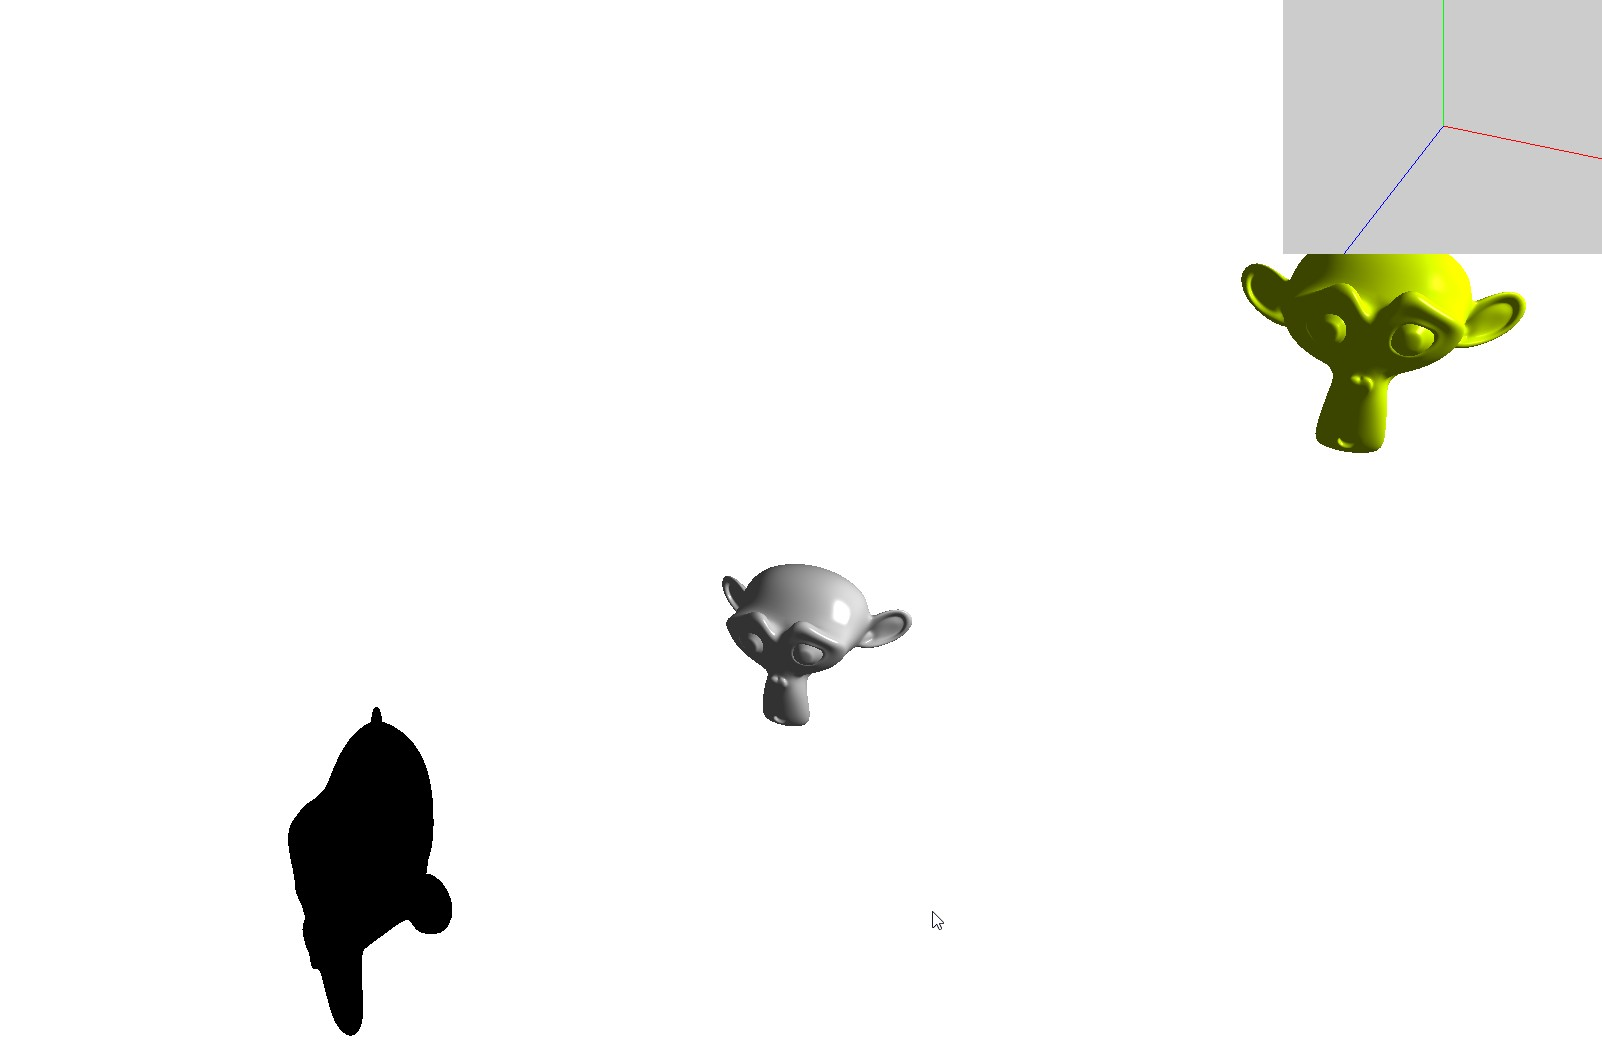
\includegraphics[width=1.0\textwidth]{figures/exercise_7}
	\end{center}
	\vspace{-4.5ex}\caption{Exercise 7 (perspective) output}
	\label{fig:exercise_7} 
\end{figure}

\begin{figure}[ht!]
	\begin{center}
		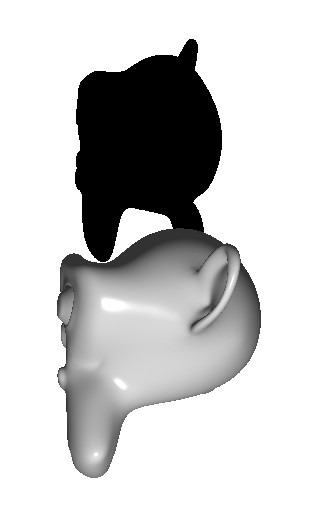
\includegraphics[width=1.0\textwidth]{figures/exercise_7_ortho}
	\end{center}
	\vspace{-4.5ex}\caption{Exercise 7 (orthogonal) output}
	\label{fig:exercise_7_ortho} 
\end{figure}